\documentclass{beamer}   % [notes=show,handout]

\usepackage{tikz}
\usepackage{graphicx}
\mode<presentation>

\usetheme{Frankfurt}%
\usecolortheme{seagull}

\definecolor{garnet}{RGB}{136,0,0}
\definecolor{clarksonGreen}{RGB}{0,52,21}

\setbeamercolor{palette primary}{fg=garnet,bg=white}
\setbeamercolor{palette secondary}{fg=clarksonGreen,bg=white}
\setbeamercolor{palette tertiary}{fg=clarksonGreen,bg=white}
\setbeamercolor{palette quaternary}{bg=clarksonGreen,fg=white}
\setbeamercolor{block title}{fg=black,bg=black!15}
\setbeamercolor{block body}{fg=black,bg=black!10}
\setbeamercolor{titlelike}{bg=garnet,fg=white} % parent=palette quaternar

\setbeamertemplate{footline}{\hspace*{.5cm}\scriptsize{\insertauthor
\hspace*{50pt} \hfill\insertframenumber\text{/}\inserttotalframenumber\hspace*{.5cm}}}

\newcommand{\R}{\mathbb{R}}


\begin{document}



\part{Introduction}
\lecture{Introduction}{Introduction}


\title{Stochastic Differential Equations}
\subtitle{Final Presentation}

\author{Liu, Sweeney, Zhou}
\institute{SUNY Potsdam and Clarkson University REU \\ with Dr. Kelly Black}
\date{July 30, 2013}

\begin{frame}[plain]
  \titlepage
  \begin{center}
  
\includegraphics[width=0.2\textwidth]{SUNYPotsdam}
  
\includegraphics[width=0.1\textwidth]{nsf_logobig}
  
\includegraphics[width=0.15\textwidth]{clarksonGreen}
\end{center}
\end{frame}

\begin{frame}
  \frametitle{Outline}
  \vspace{-5mm}
  \tableofcontents[pausesection,hideallsubsections]
\end{frame}





\section{Introduction}

\begin{frame}
    \frametitle{Background}
	\begin{itemize}
		\item Insurance
			\item\item Low risk investments with government bonds
			\item\item Government regulated
		\item Deer
	\end{itemize}

\end{frame}







\section{Population Biology}

\begin{frame}
    \frametitle{Deer}
\end{frame}

\begin{frame}
    \frametitle{Logistic Equation}
	\begin{eqnarray}
		\frac{dx}{dt} &=& rx(k-x)
	\end{eqnarray}
	\begin{itemize}
		\item $k$ - carrying capacity
		\item 
	\end{itemize}
\end{frame}

\begin{frame}
    \frametitle{State and Federal Statistics}
\end{frame}






\section{Insurance}

\begin{frame}
    \frametitle{State Regulations and Bond Funds}
\end{frame}






\section{Model}

\begin{frame}
    \frametitle{Stochastics}
	\begin{itemize}
		\item Brownian Motion (Random Walks) - $W(t)$
		\item Properties
	\begin{enumerate}[i]
		\item $W(t)$ is continuous
		\item $W(t)$ is no where differentiable
		\item If $t_{1}<t_{2}<t_{3}<t_{4}$, \\
			$W(t_{1}), W(t_{2})-W(t_{1}),  W(t_{3})-W(t_{4})$ are independent random variables
		\item If $0 \le s\le t$ then $W(t)-W(s) \sim N(0, t-s)$
	\end{enumerate}
		\item Gaussian White ``Noise" - $dW$
	\end{itemize}
%%%%%%%%%% Brownian Motion, Gaussian White Noise
\end{frame}



\begin{frame}
    \frametitle{Models}
	\begin{eqnarray}
		dx &=& \tilde{r} x \left( 1- \frac{x}{\tilde{f}}\right) dt +\alpha x \, dW \\
		dm &=& ( \rho m - \beta x + P) dt - \gamma x \, dW
	\end{eqnarray}
	\begin{itemize}
		\item Known Parameters - $\tilde{r}$, $\tilde{f}$, $\rho$, $\beta$
		\item Unknown Parameters - $\alpha$, $\gamma$, $P$
	\end{itemize}
\end{frame}




\section{Numerics}

\begin{frame}
   \frametitle{Approximation}
%%%%%%%%%Include figure
	\begin{eqnarray*}
		dX &=& f(X) \, dt + g(X) \, dW \\
	\end{eqnarray*}
	\begin{center}
		$X_{j} =$ approximation of $X(t_{j})$
	\end{center}
\end{frame}


\begin{frame}
    \frametitle{Methods of Approximations}
	Euler-Maruyama Method - $O(\Delta t^{1})$
	\begin{eqnarray*}
		X_{j} &=& X_{j-1} + f(X_{j-1})\triangle t+ g(X_{j-1})(W(\tau_{j})-W(\tau_{j-1})) \\
		 j &=& 1,2,... ,L \\
	\end{eqnarray*}
	Milstein Method - $O(\Delta t^{1.5})$
	\begin{eqnarray*}

		X_{j} &=& X_{j-1} + \triangle tf(X_{j-1}) + g(X_{j-1})(W(\tau_{j})-W(\tau_{j-1})) 	\nonumber\\ 
		&& + \frac{1}{2} g(X_{j-1})g'(X_{j-1})((W(\tau_{j})-W(\tau_{j-1}))^{2}-\triangle t)\\
		 j &=& 1,2,... ,L \\
	\end{eqnarray*}
\end{frame}


\begin{frame}
    \frametitle{Benchmark}
	\framesubtitle{Paths}
\vspace{-5mm}
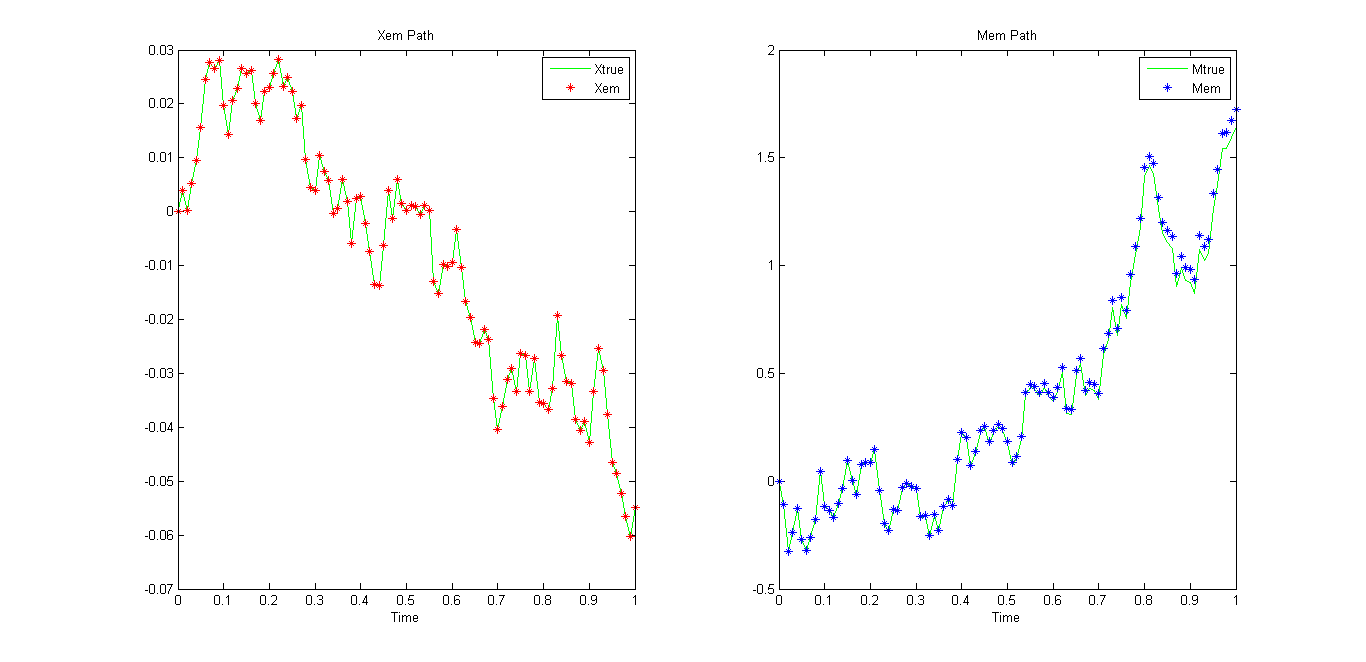
\includegraphics[height=6cm,width=12cm]{testpaths} 
\end{frame}


\begin{frame}
    \frametitle{Benchmark}
	\framesubtitle{Histogram}
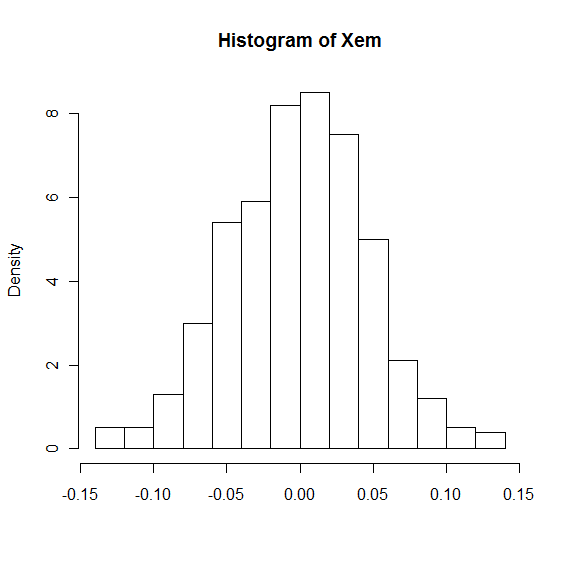
\includegraphics[height=6cm,width=6cm]{testhistX}
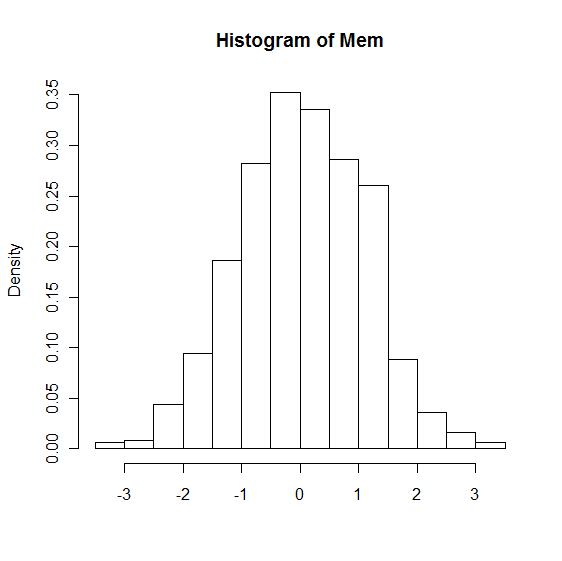
\includegraphics[height=6cm,width=6cm]{testhistM}
\end{frame}


\begin{frame}
    \frametitle{Benchmark}
	\framesubtitle{Confidence Interval}
\begin{center}
	$\bar{x} \pm t_{(\alpha /2, df=n-1)} \frac{s}{\sqrt{n}}$
\end{center}
\begin{eqnarray*}
	E[X] = 0 && E[M] = 0 \\
	Var[X] = 0.0025  && Var[M] = 1
\end{eqnarray*}
95 \% Confidence Interval
\begin{itemize}
	\item $\bar{X}$ (-0.0088, 0.0067)
	\item $\bar{M}$ (-0.137, 0.217)
\end{itemize}
\end{frame}


\begin{frame}
    \frametitle{Parameter Space}
%%%%%%%%%% Include 3D plot of parameter space
\end{frame}









\section{Results}

\begin{frame}
    \frametitle{Results}
\vspace{-4mm}
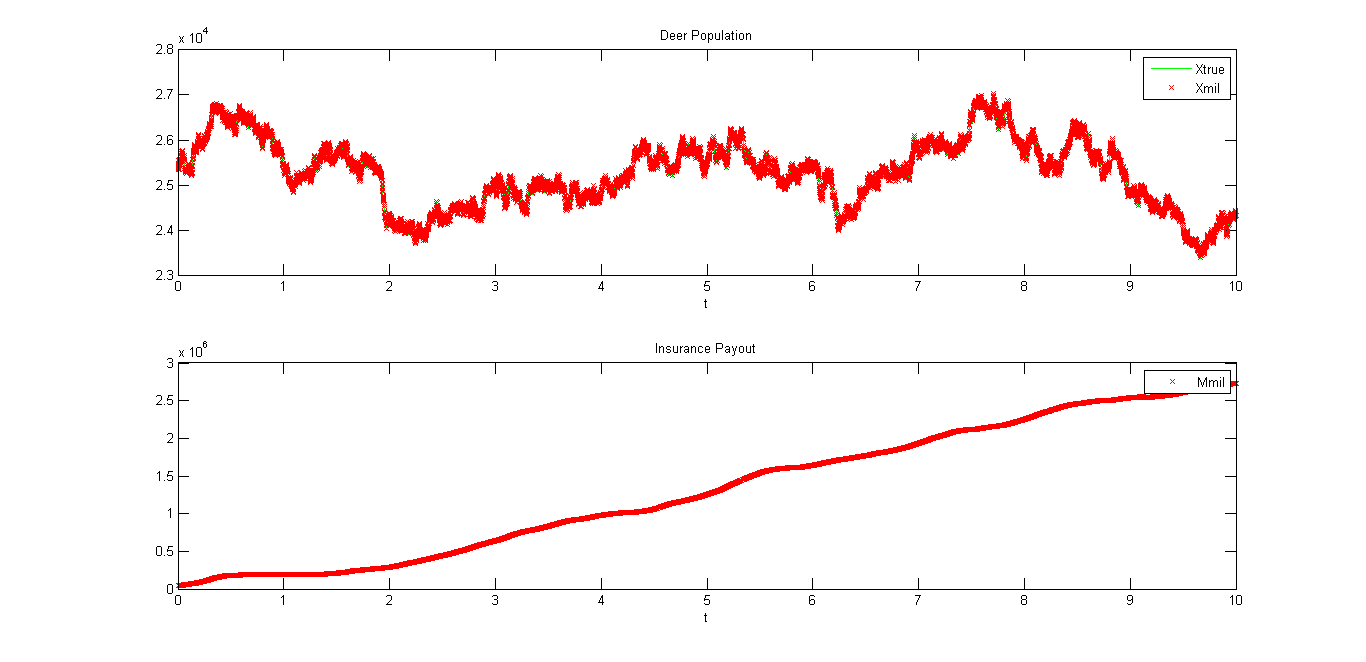
\includegraphics[height=8cm,width=12cm]{deerins}
\end{frame}






\section{Conclusions}

\begin{frame}
    \frametitle{Conclusion}
\end{frame}









\section{References}

\begin{frame}
    \frametitle{References}
\end{frame}



\section{Acknowledgements}

\begin{frame}
    \frametitle{Acknowledgements}
	Thanks to Dr. Joel Foisy, Dr. Kelly Black and NSF (NSF \# 1262737) for their support and involvement in this program.
\end{frame}



\end{document}
